\documentclass[12pt, letterpaper]{article}
\usepackage{graphicx} % Import graphics
\usepackage{float} % Figure placement with H
\usepackage{caption}
\usepackage{subcaption} % for subfigure stuff 
\usepackage[table]{xcolor} % for making tables look good
\usepackage{tabularx}
\usepackage{geometry}
\graphicspath{{figures/}} % Configure the graphicx package

\geometry{
  left=0.5in,
  right=0.5in,
  top=0.5in,
  bottom=0.5in
}

\title{M1 Layer 2/3 Brief Network Summary}
%\author{Greg Glickert}
\date{Aug 1, 2024}

\begin{document}
\pagestyle{empty} % removes page number on rest of pages
\maketitle
\thispagestyle{empty} % removes page number on first page

\section*{Single Cells}
We will use a 87,9,4 ratios for PN,FSI and LTS cells in our model. 
The ratio of excitatory:inhibitory neurons is 87:13\cite{Lefort2009}. 
The FSI:LTS cells ratio is 70:30\cite{Kätzel2010}\cite{Wall2016}.
The network consists of 10,000 cells, the same size as Ziao's model. 
The PN cell was adapted from the L5 CP cell to make it more L2/3-like\cite{Hirai2012}. 
The interneurons use the same template as the L5 model.

\begin{table}[H]
  \centering
  \caption{Cell properties}
  \begin{tabularx}{\textwidth}{|X|X|X|X|X|X|X|}
  \hline
  Cell & Apical Length (um) & V-Rest (mV) & R\_in (Mohms) & Tau\_m (ms) & Rheobase (pA) & FI curve slope \\ \hline
  PN:  & 324\cite{Ledergerber2010} & -77.11\cite{Hirai2012} & 112.85\cite{Hirai2012}  & 14.87\cite{Hirai2012}  & 200\cite{Hirai2012}   & $\sim$100\cite{Hirai2012}      \\ \hline
  FSI: & 150               & -69.94\cite{Tanaka2011}     & 223.12\cite{Tanaka2011}       & 12.03\cite{Tanaka2011}      & 40           & $\sim$500      \\ \hline
  LTS: & 250               & -70.00\cite{Tanaka2011}     & 289.81\cite{Tanaka2011}       & 19.43\cite{Tanaka2011}      & 40           & $\sim$160      \\ \hline
  \end{tabularx}
\end{table}

\section*{Synapses}
The synapses are the same as Ziao's L5 model except the reversal potential of the FSI2PN and LTS2PN synapses has been updated to -75mV to better match biological data\cite{Beierlein2003}.

\begin{table}[H]
  \centering
  \caption{Synaptic Properties from literature}
  \begin{tabularx}{\textwidth}{|X|X|X|X|X|X|X|X|X|}
    \hline
    Cell Pair & latency                        & amp                             & rise time                       & decay time                     & half width                     & PPR \\ \hline
    PN2PN     & 1.6$\pm$0.3\cite{Morishima2011}  & 32.2$\pm$27.4\cite{Morishima2011} & 1.2$\pm$0.45\cite{Morishima2011}  &  6.9$\pm$1.9\cite{Morishima2011} & 12.3$\pm$2.2\cite{Beierlein2003} & 1.27$\pm$0.34\cite{Morishima2011} \\ \hline
    PN2FSI    & 1.3$\pm$0.38\cite{Morishima2017} & 32.0$\pm$25.5\cite{Morishima2017} & 0.56$\pm$0.18\cite{Morishima2017} & 3.6$\pm$1.2\cite{Morishima2017}  & 4.9$\pm$1.6\cite{Beierlein2003}  & 1\cite{Morishima2017} \\ \hline
    PN2LTS    & 1.5$\pm$0.51\cite{Morishima2017} & 4.6$\pm$3.5\cite{Morishima2017}   & 1.2$\pm$0.47\cite{Morishima2017}  & 5.1$\pm$2.0\cite{Morishima2017}  & 8.9$\pm$2.9\cite{Beierlein2003}  & 2\cite{Morishima2017} \\ \hline
    FSI2PN    & NA                               & 1.1$\pm$0.8\cite{Beierlein2003}   & 1.5$\pm$0.7\cite{Beierlein2003}   & NA                               & 24$\pm$10.8\cite{Beierlein2003}  & NA \\ \hline
    LTS2PN    & NA                               & 0.48$\pm$0.45\cite{Beierlein2003} & 2.1$\pm$1.0\cite{Beierlein2003}   & NA                               & 22.6$\pm$13.7\cite{Beierlein2003}& NA \\ \hline
    FSI2FSI   & NA                               & 23.9$\pm$7.8pA\cite{Galarreta2002}& 0.89$\pm$0.04\cite{Galarreta2002} & 5.9$\pm$0.5\cite{Galarreta2002}  & NA                               & 0.66\cite{Galarreta2002}\\ \hline
    LTS2FSI   &                                  &                                   &                                   &                                  &                                  &                          \\ \hline
    FSI2LTS   &                                  &                                   &                                   &                                  &                                  &                          \\ \hline
    LTS2LTS   &                                  &                                   &                                   &                                  &                                  &                          \\ \hline     
  
  \end{tabularx}
  \label{tab:syn_prop}
\end{table}



\begin{table}[H]
  \centering
  \caption{Synaptic Properties in Network *matches literature}
  \begin{tabularx}{\textwidth}{|X|X|X|X|X|X|X|X|X}
    \hline
    Cell Pair & baseline & sign & latency & amp & rise time & decay time & half width & PPR \\ \hline
    PN2PN & 0.1734 & -1.0000 & 1.6500* & 0.0155 & 1.2000* & 7.1844* & 10.1000* & 1.3474* \\ \hline
    PN2FSI & 0.0376 & -1.0000 & 1.6500* & 0.0068 & 0.5500* & 3.6355* & 4.9500* & 0.9974* \\ \hline
    PN2LTS & 0.0345 & -1.0000 & 1.6500* & 0.0026 & 1.2000* & 5.1287* & 6.9000* & 2.2518* \\ \hline
    FSI2PN & 0.1734 & 1.0000 & 0.0250 & 0.0171 & 0.2250 & 7.0431 & 5.6750 & 1.0389 \\ \hline
    LTS2PN & 0.1734 & 1.0000 & 0.0250 & 0.0043 & 1.1250 & 31.5004 & 24.7750 & 2.1033 \\ \hline
    FSI2FSI & -0.0691 & 1.0000 & 1.6500 & 0.0750 & 0.3250 & 5.0295 & 5.8500 & 0.7252 \\ \hline
    LTS2FSI & -0.0691 & 1.0000 & 1.6500 & 0.0060 & 1.4250 & 20.1433 & 18.8250 & 1.7405 \\ \hline
    FSI2LTS & 0.0345 & 1.0000 & 1.6500 & 0.0675 & 0.3250 & 5.0295 & 5.8500 & 0.7252 \\ \hline
    LTS2LTS & 0.0345 & 1.0000 & 1.6500 & 0.0113 & 1.4250 & 20.1433 & 18.8250 & 1.7405 \\ \hline
  \end{tabularx}
  \label{tab:syn_prop}
\end{table}


\begin{table}[H]
  \centering
  \caption{Synaptic Parameters}
  \begin{tabularx}{\textwidth}{|X|X|X|X|X|X|X|X|X}
    \hline
    Cell Pair & initW & tau r AMPA & tau d AMPA & Use & Dep & Fac & level of detail & e \\ \hline
    PN2PN & 3.2000 & 0.2000 & 5.2000 & 0.3700 & 31.7000 & 519.0000 & AMPA NMDA STP & 0 \\ \hline
    PN2FSI & 3.1000 & 0.4000 & 2.9000 & 0.0350 & 500.0000 & 0.0000 & AMPA NMDA STP & 0 \\ \hline
    PN2LTS & 1.0000 & 0.4000 & 3.9000 & 0.0500 & 0.0000 & 200.0000 & AMPA NMDA STP & 0 \\ \hline
    FSI2PN & 3.8000 & 0.2000 & 7.0000 & 0.3000 & 400.0000 & 0.0000 & GABA A STP & -75.0  \\ \hline
    LTS2PN & 1.0000 & 0.9000 & 30.0000 & 0.3000 & 25.0000 & 200.0000 & GABA A STP & -75.0 \\ \hline
    FSI2FSI & 10.0000 & 0.2000 & 5.0000 & 0.3000 & 400.0000 & 0.0000 & GABA A STP & -75.0 \\ \hline
    LTS2FSI & 0.8000 & 0.9000 & 20.0000 & 0.3000 & 25.0000 & 200.0000 & GABA A STP & -75.0 \\ \hline
    FSI2LTS & 15.0000 & 0.2000 & 5.0000 & 0.3000 & 400.0000 & 0.0000 & GABA A STP & -75.0 \\ \hline
    LTS2LTS & 2.5000 & 0.9000 & 20.0000 & 0.3000 & 25.0000 & 200.0000 & GABA ASTP & -75.0 \\ \hline
  \end{tabularx}
  \label{tab:syn_prop}
\end{table}





\section*{Connectivity}
The network connectivity has been altered from Ziao's L5 model. 
The PN2PN\cite{Holmgren2003}, PN2FSI\cite{Holmgren2003},FSI2PN\cite{Holmgren2003}, and LTS2PN\cite{Fino2011} connection functions have been modified based on L2/3 data. 
The interneuron to interneuron and PN2LTS functions have not been altered.
However since the cell ratios have been altered the same connection rules will give slightly different connection numbers. 
We may need to change the PN2LTS connection functions to update all connections that "touch" a PN.
I have not yet found a good PN2LTS connection paper, but i am sure one is out there just have to go digging.





\begin{figure}[H]
  \centering
  \begin{subfigure}{0.4\textwidth}
    \centering
    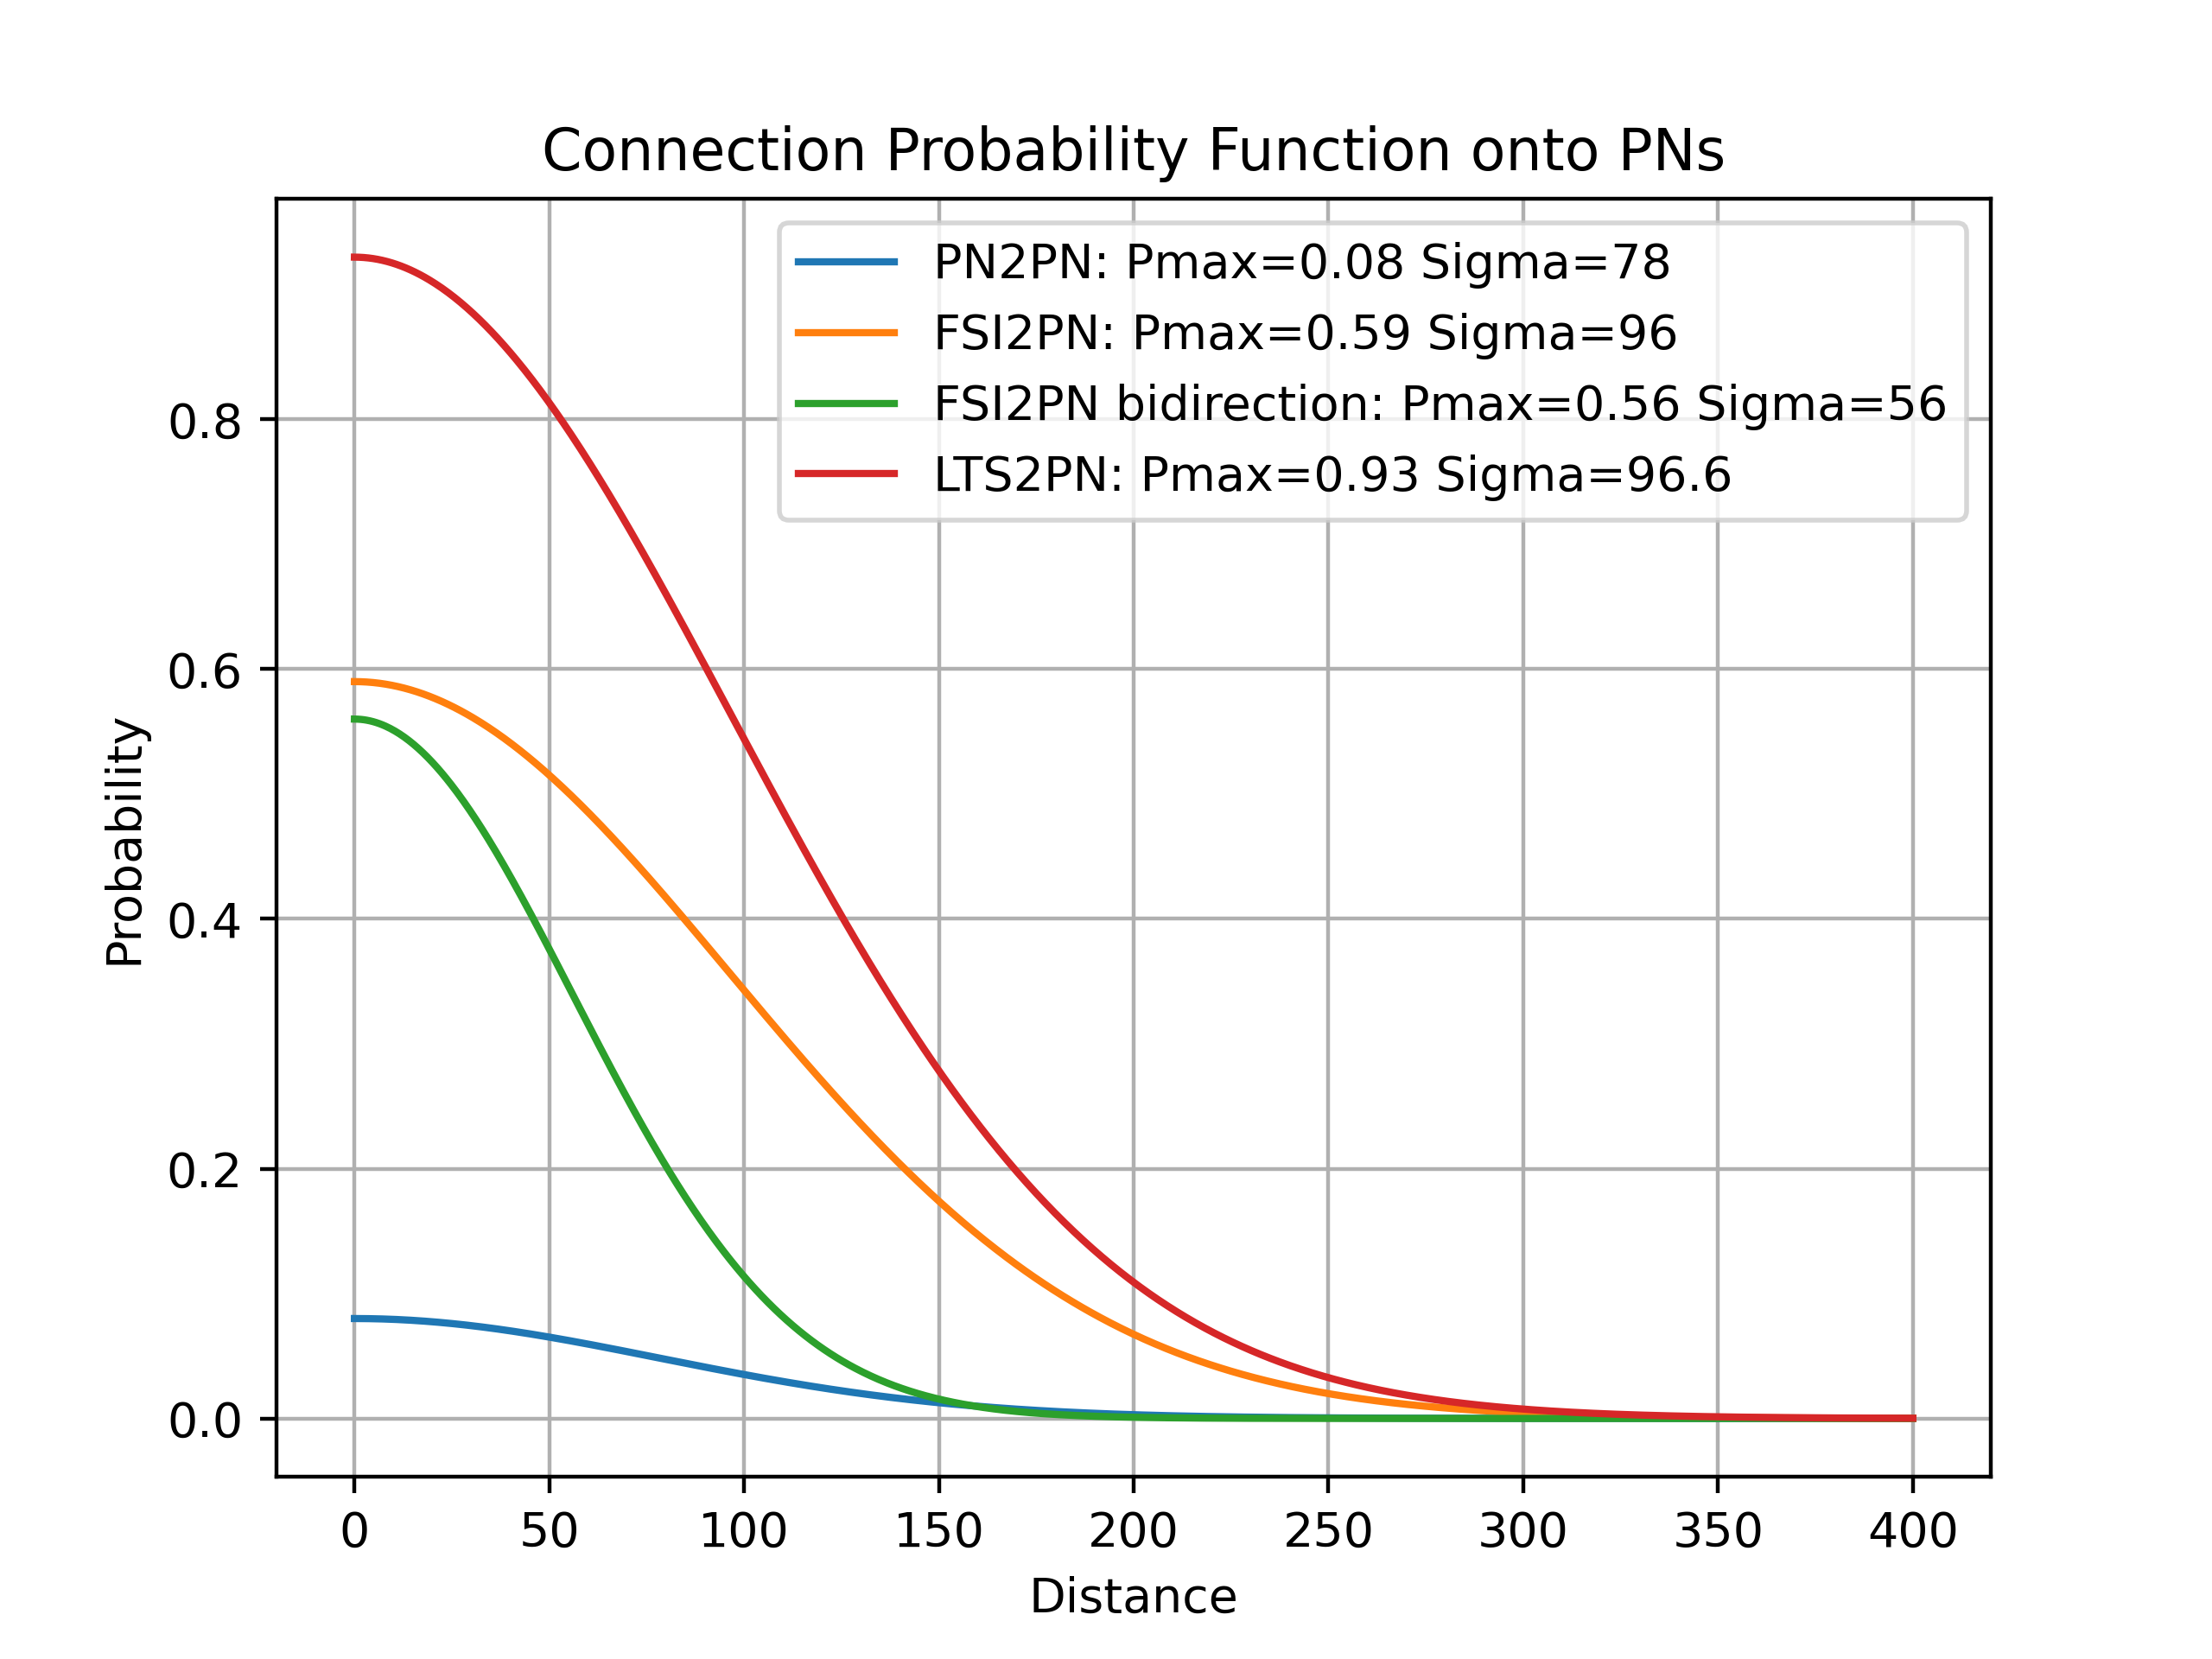
\includegraphics[width=\linewidth]{connections/onto-pn-functions}
    \caption{functions for connecting to PN cells}
    \label{fig:Gaussian PN}
  \end{subfigure}
  \begin{subfigure}{.4\textwidth}
    \centering
    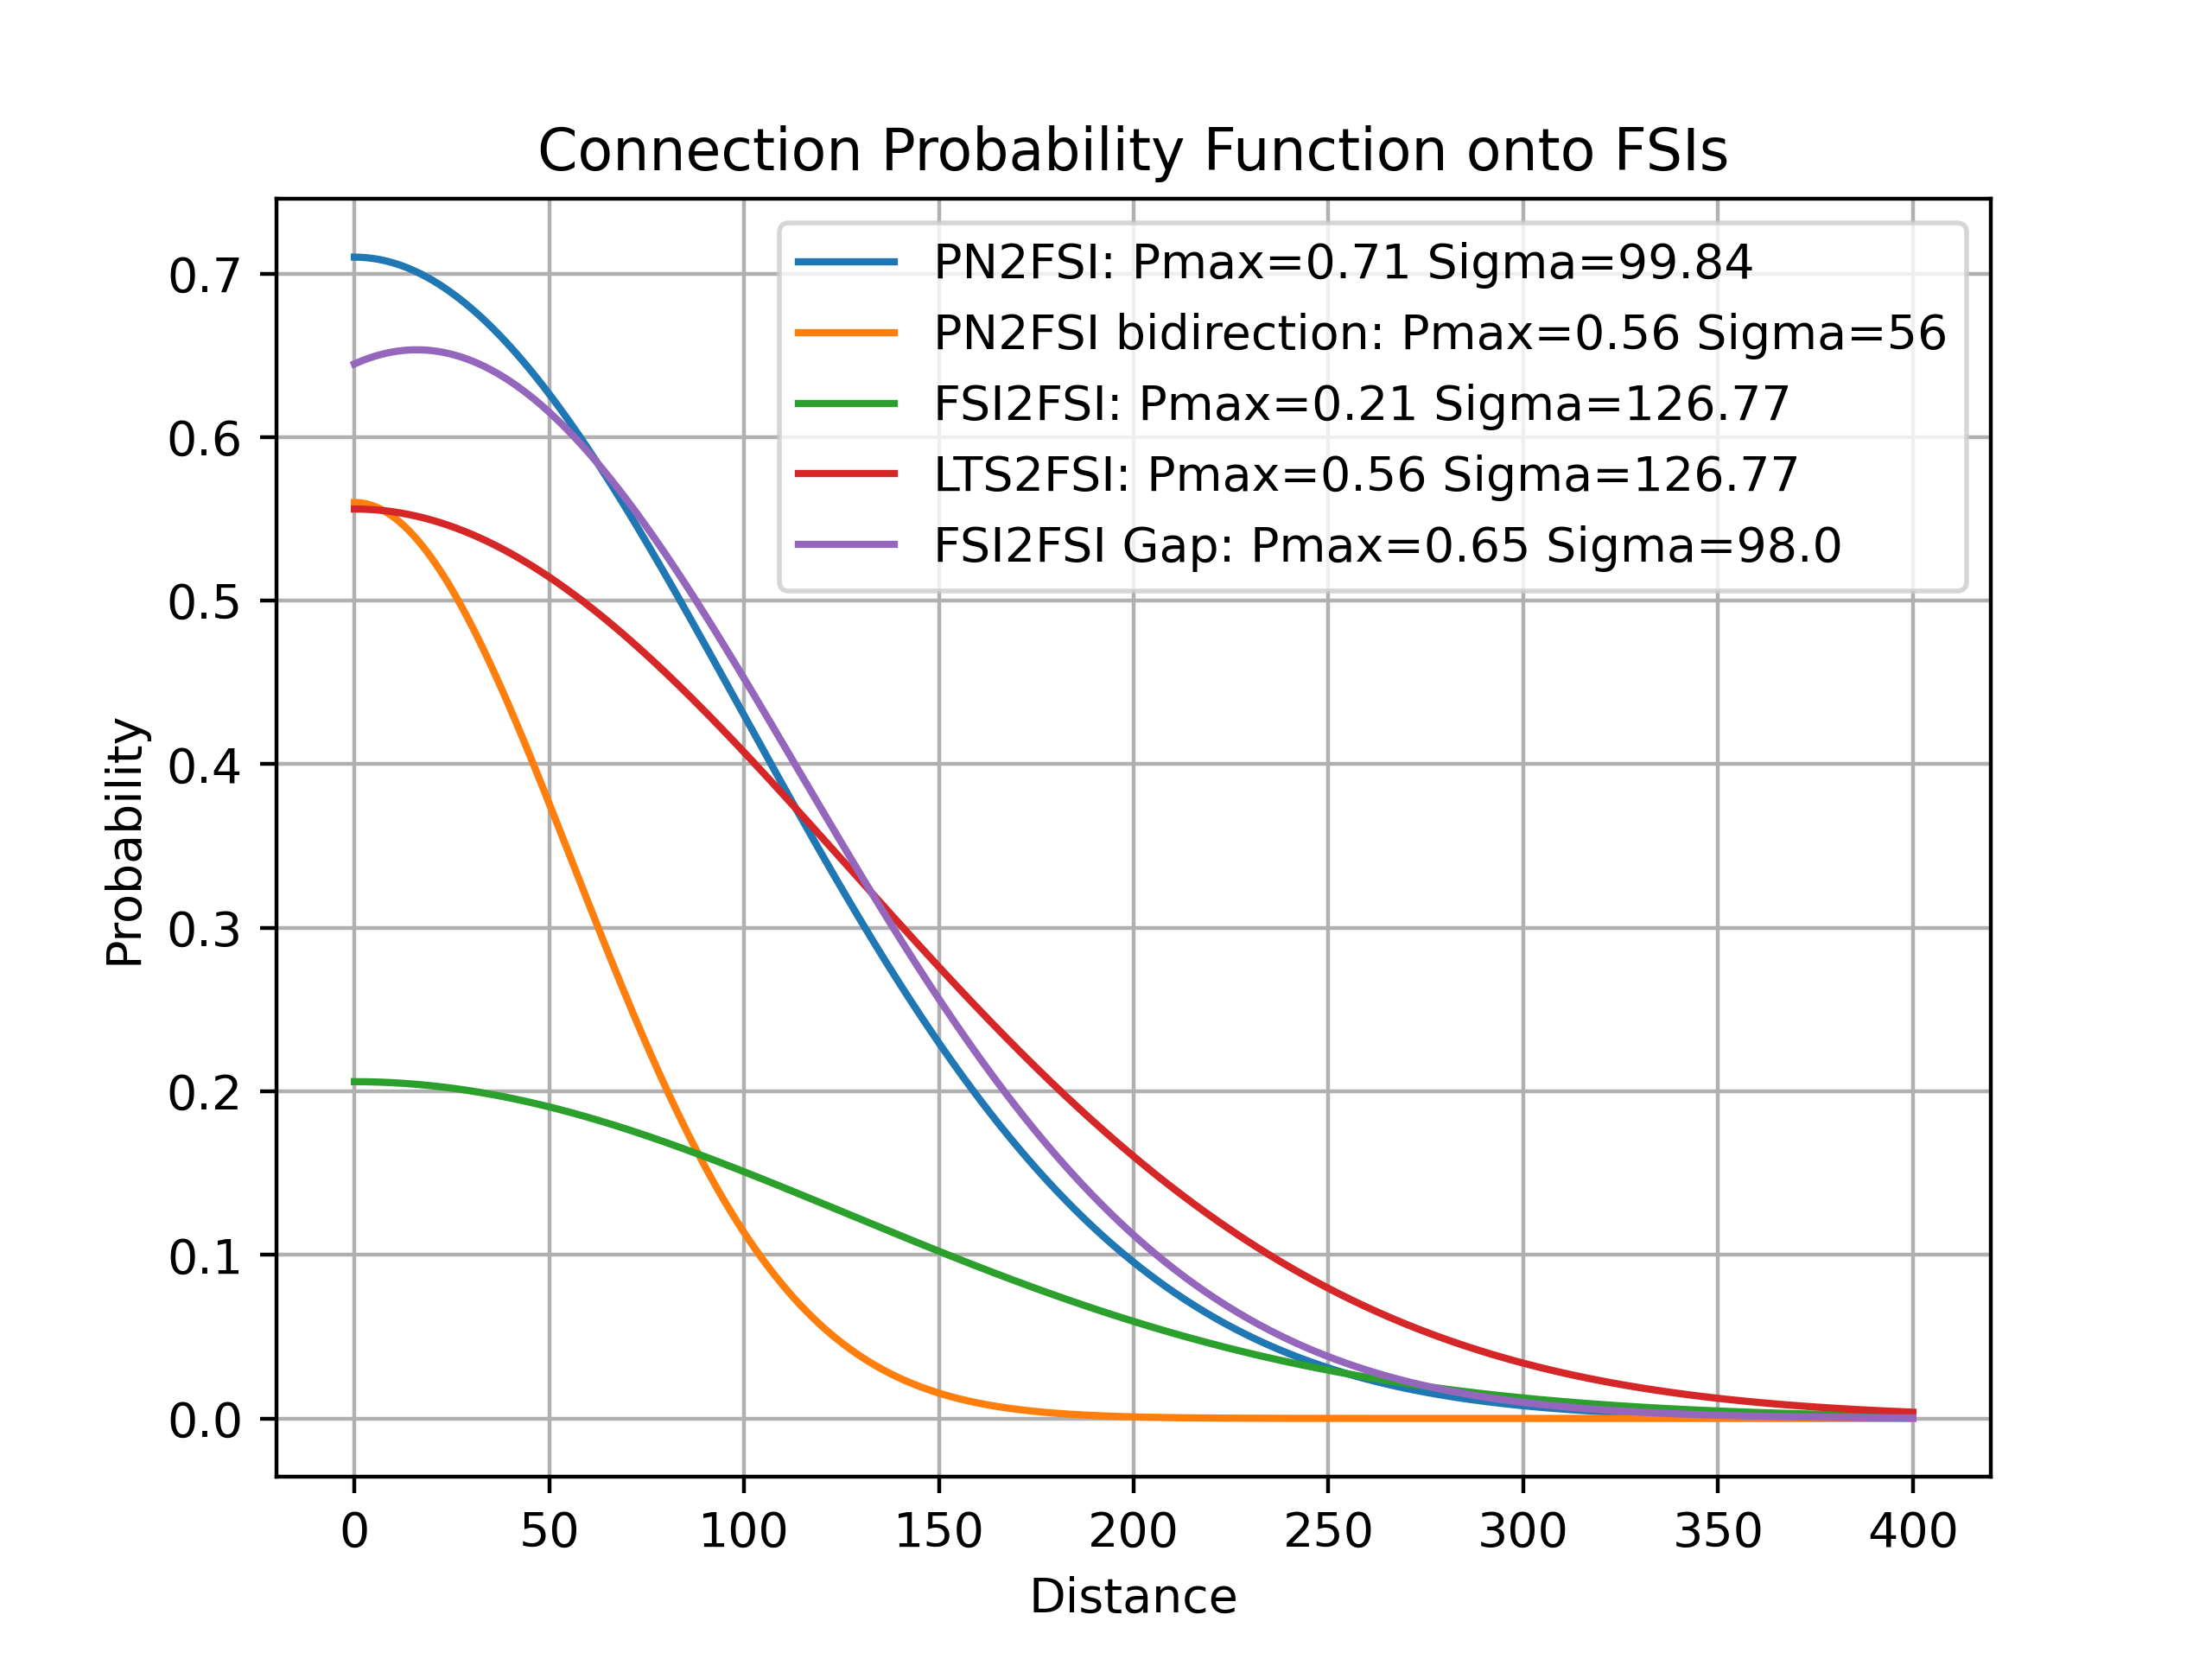
\includegraphics[width=\linewidth]{connections/onto-fsi-functions}
    \caption{functions for connecting to FSI cells}
    \label{fig:Gaussian FSI}
  \end{subfigure}
  \begin{subfigure}{.4\textwidth}
    \centering
    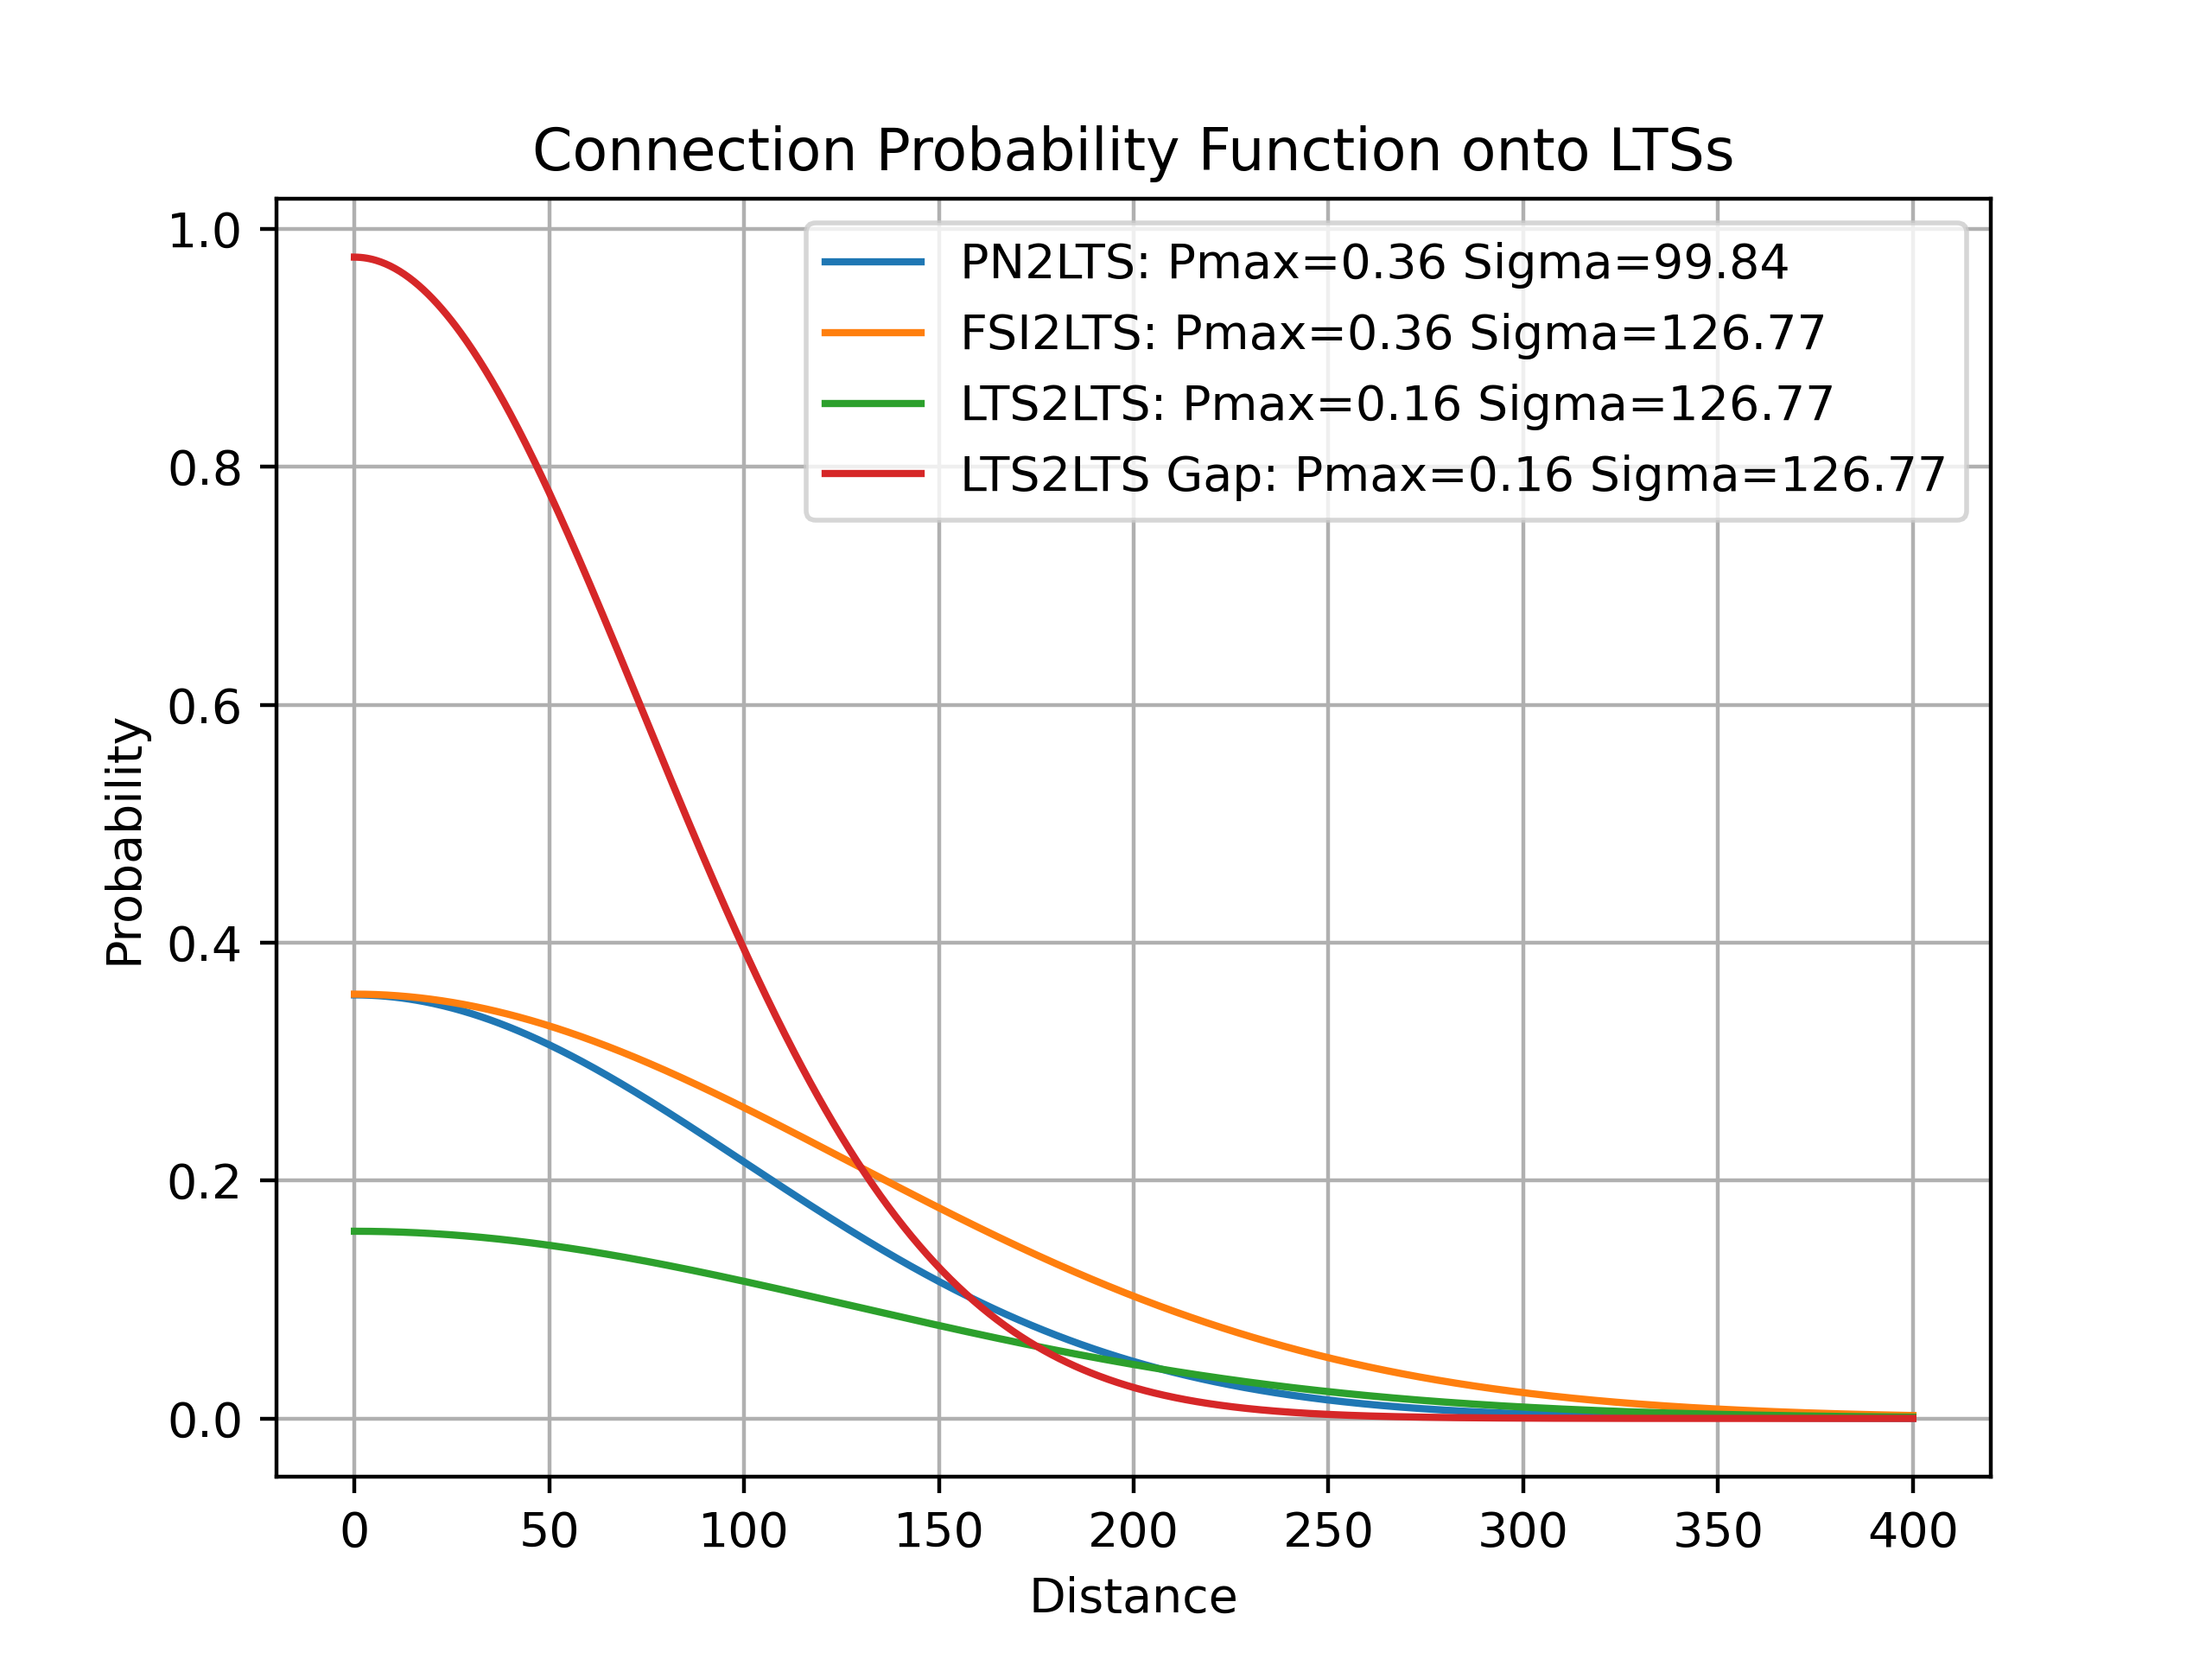
\includegraphics[width=\linewidth]{connections/onto-lts-functions}
    \caption{functions for connecting to LTS cells}
    \label{fig:Gaussian LTS}
  \end{subfigure}
  \caption{Gaussian connection functions for each cell type}
  \label{fig:Gaussian connection functions}
\end{figure}


\begin{figure}[H]
    \centering
    \begin{subfigure}{.5\textwidth}
      \centering
      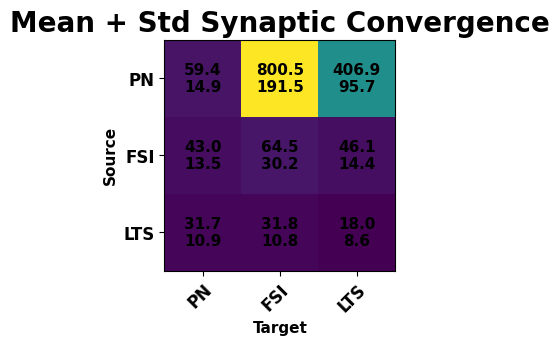
\includegraphics[width=\linewidth]{connections/bio-connvergence}
      \caption{Biophysical Convergence}
      \label{fig:sub1}
    \end{subfigure}
    \begin{subfigure}{.5\textwidth}
      \centering
      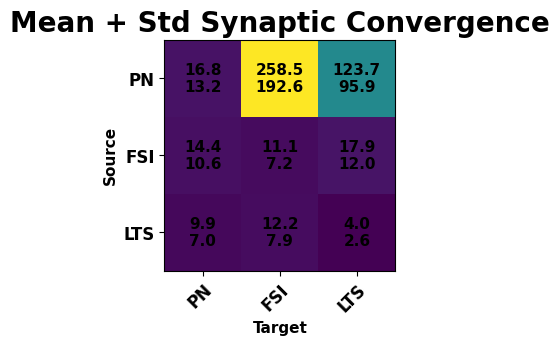
\includegraphics[width=\linewidth]{connections/shell-convergence}
      \caption{Shell Convergence}
      \label{fig:sub2}
    \end{subfigure}
    \begin{subfigure}{.5\textwidth}
      \centering
      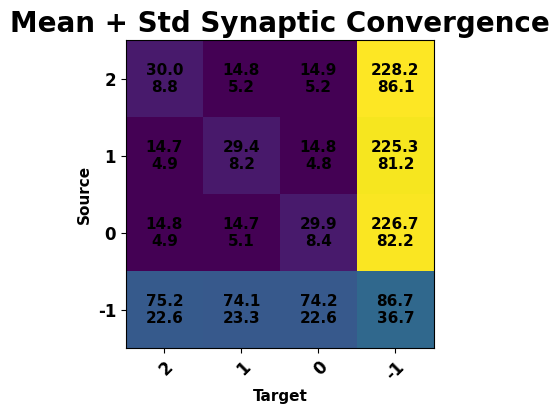
\includegraphics[width=\linewidth]{connections/assembly-convergence}
      \caption{Assembly Convergence}
      \label{fig:sub3}
    \end{subfigure}
    \caption{Convergence Matrix}
    \label{fig:test}
\end{figure}

\begin{figure}[H]
    \centering
    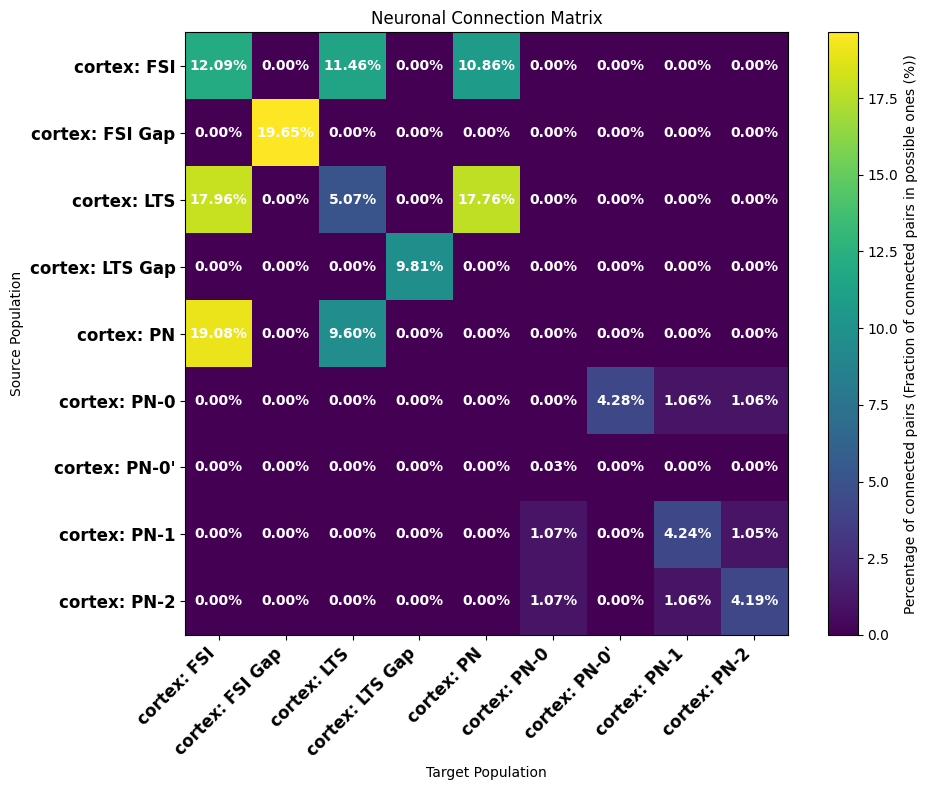
\includegraphics[width=\textwidth]{connections/percent-connections}
    \caption{Percent Connectivity of Possible Connections (Factoring in Distance rules)}
    \label{fig:percentconns}
\end{figure}

\section*{Model Output}

\subsection*{Baseline}

\begin{figure}[H]
  \centering
  \begin{subfigure}{\textwidth}
    \centering
    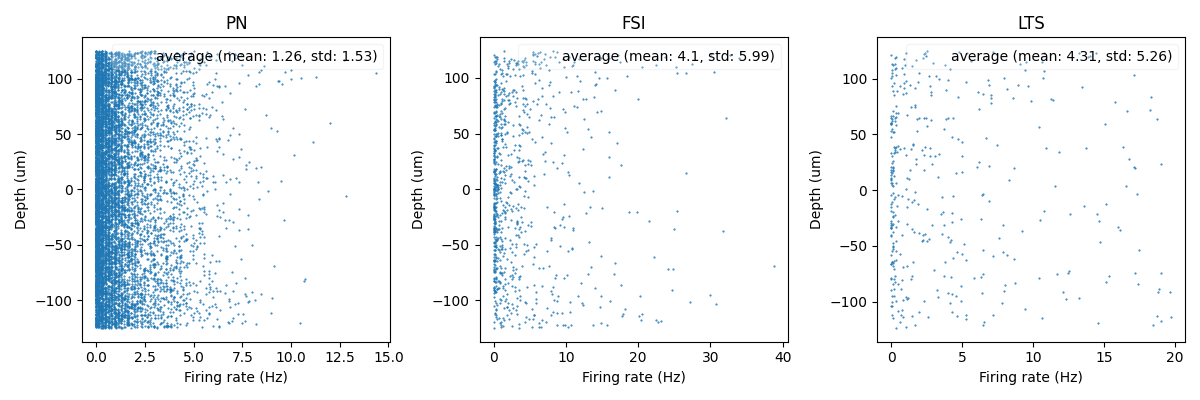
\includegraphics[width=\textwidth]{output/baseline-spikes}
    \caption{Firing Rate during Baseline}
    \label{fig:baseline-spikes}
  \end{subfigure}
  \begin{subfigure}{\textwidth}
    \centering
    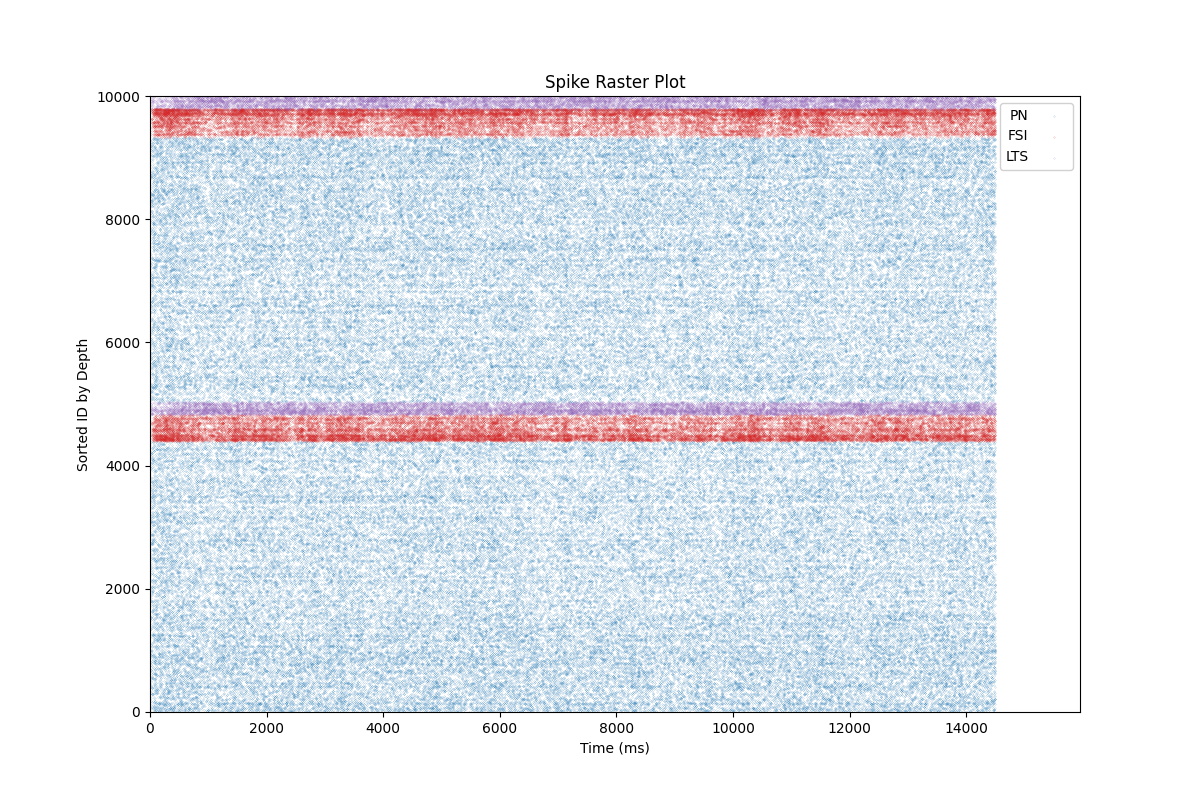
\includegraphics[width=\textwidth]{output/baseline-raster}
    \caption{Raster}
    \label{fig:baseline-raster}
  \end{subfigure}
  \caption{Firing Rate Analysis for Baseline}
\end{figure}

\begin{figure}[H]
    \centering
    \begin{subfigure}{.75\textwidth}
      \centering
      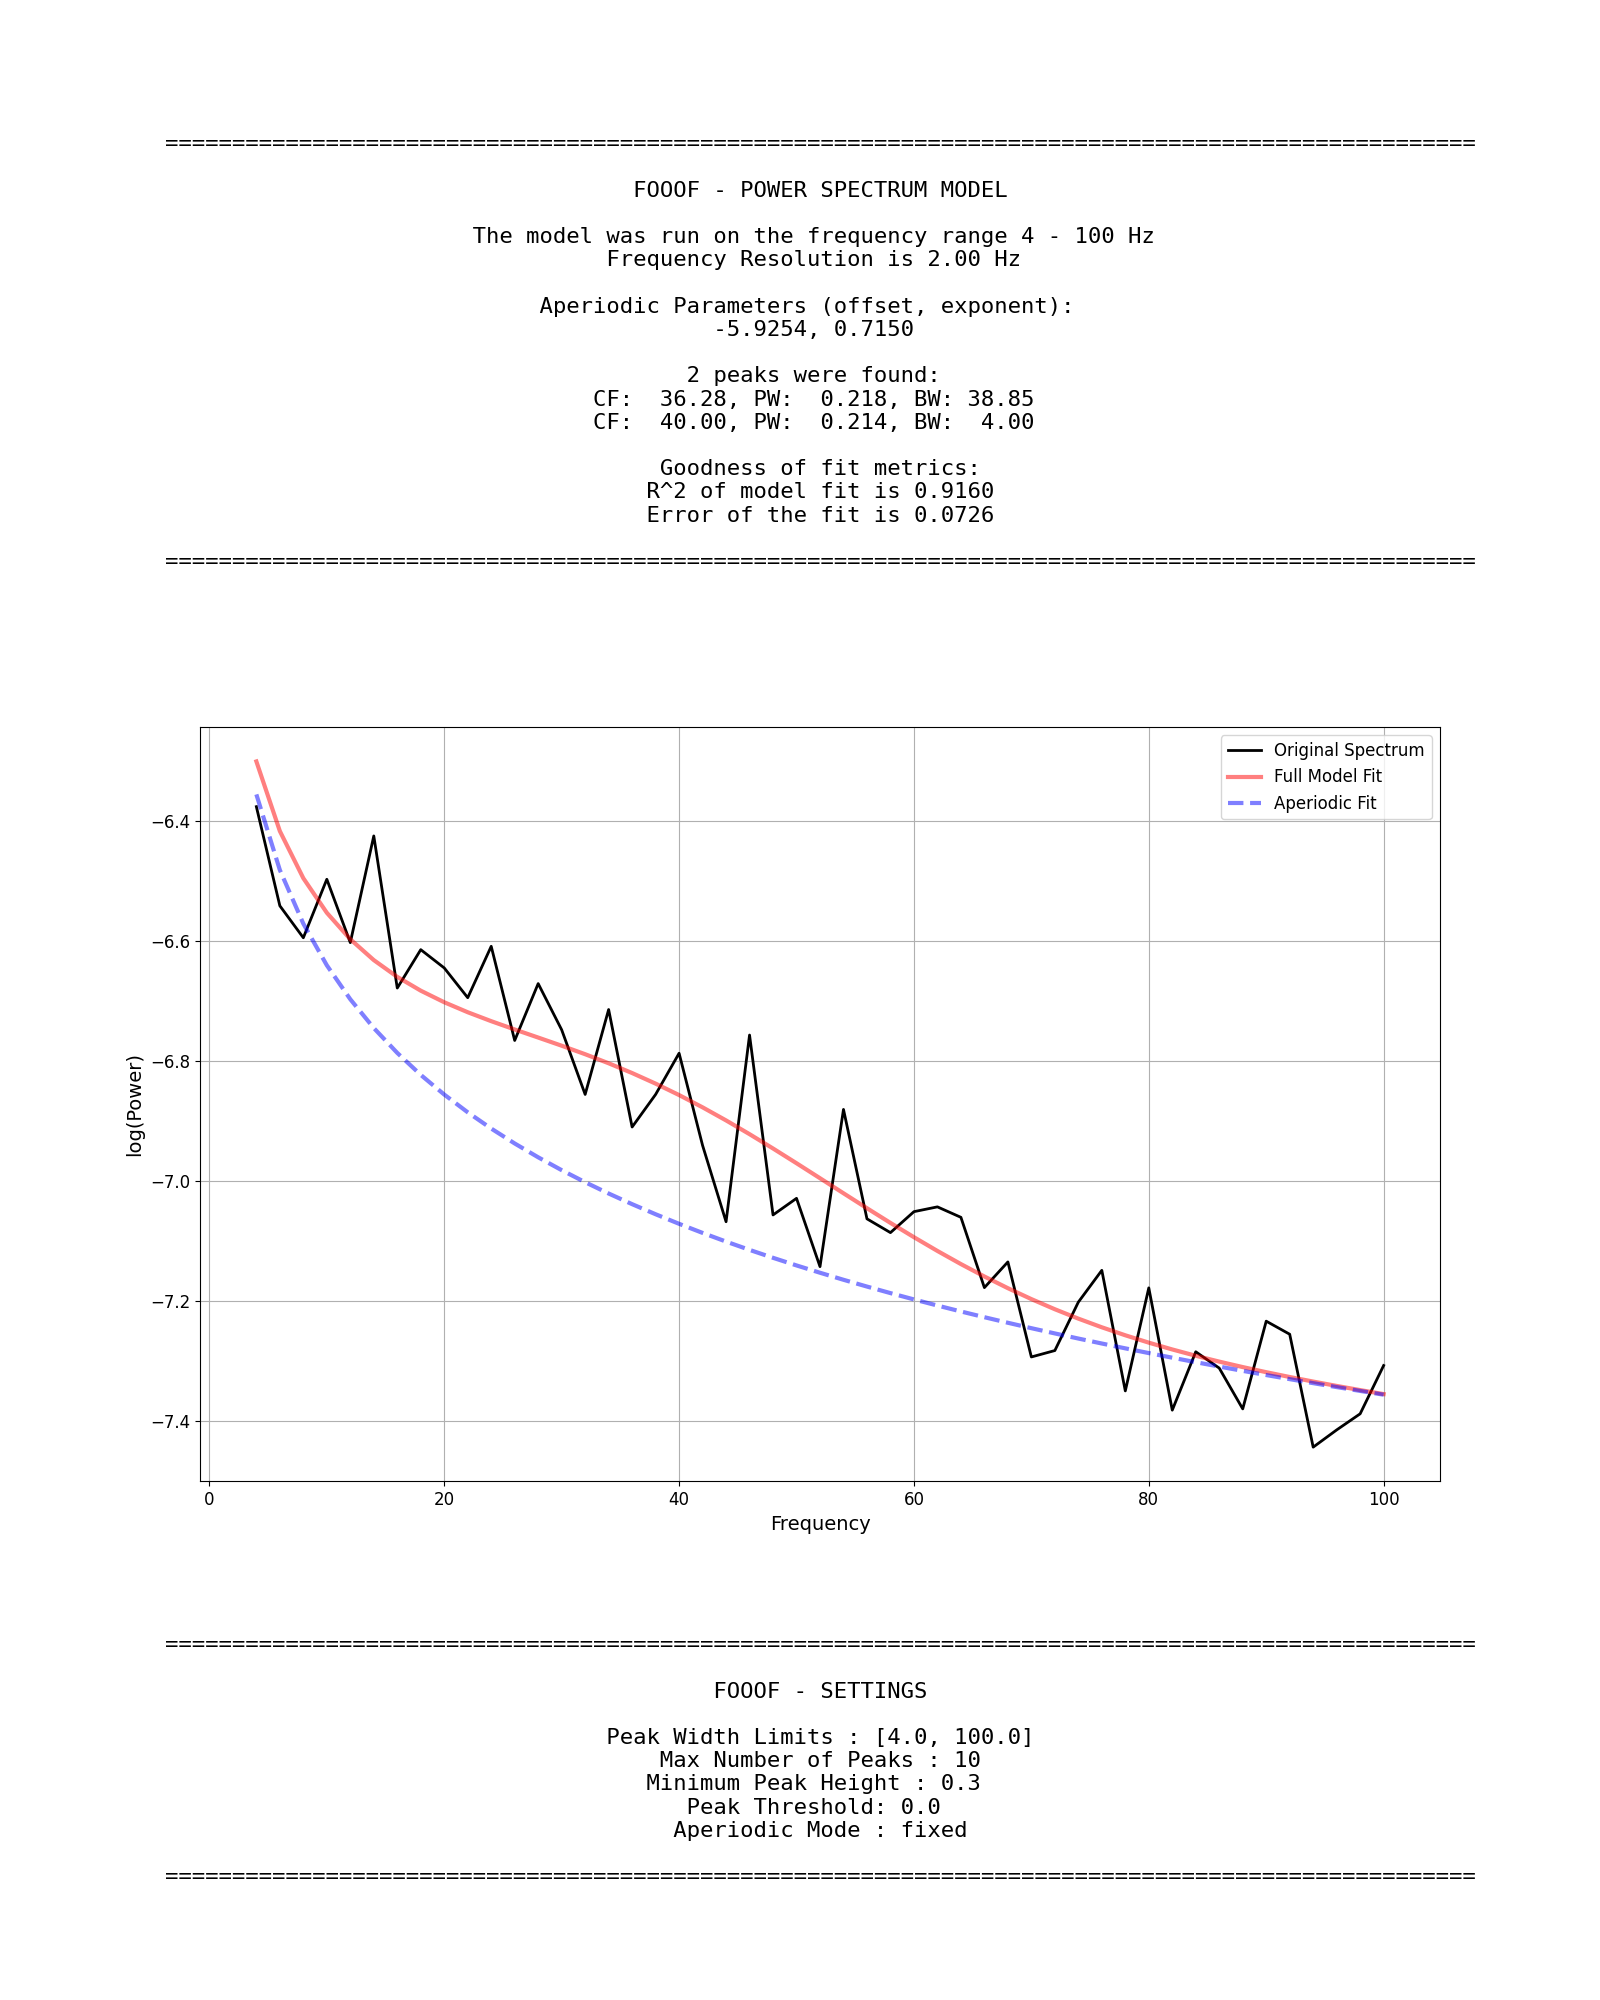
\includegraphics[width=\textwidth]{output/baseline-psd}
      \caption{Fooof Report}
      \label{fig:baseline-psd}
    \end{subfigure}
    \begin{subfigure}{.75\textwidth}
      \centering
      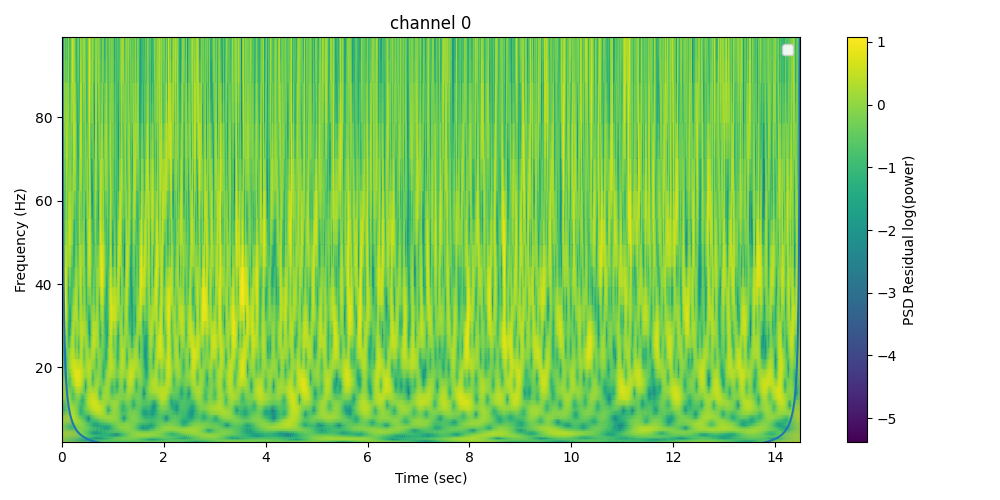
\includegraphics[width=\textwidth]{output/baseline-spectrogram}
      \caption{Spectrogram}
      \label{fig:baseline-spectrogram}
    \end{subfigure}
    \caption{Spectral Analysis for Baseline}
\end{figure}

\subsection*{Short Pulse}

\begin{figure}[H]
  \centering
  \begin{subfigure}{\textwidth}
    \centering
    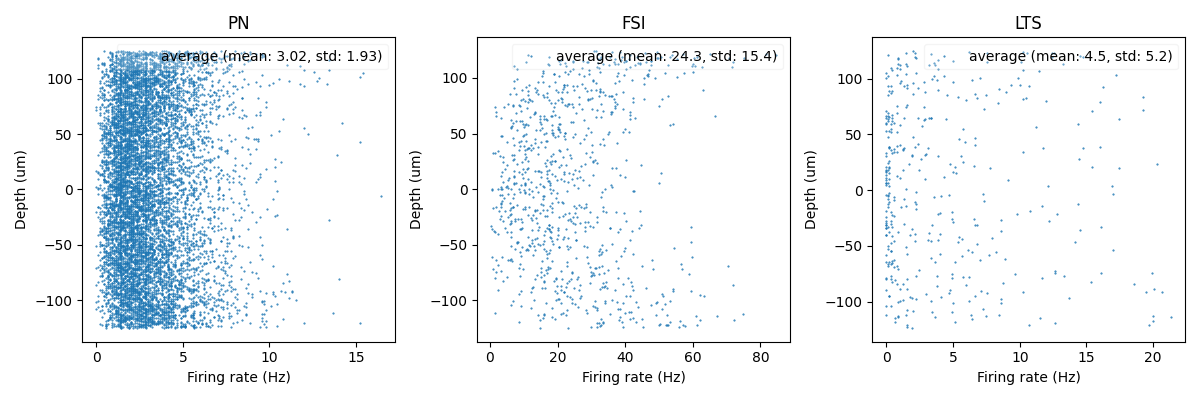
\includegraphics[width=\textwidth]{output/short-spikes}
    \caption{Firing Rate during Short Pulse}
    \label{fig:short-spikes}
  \end{subfigure}
  \begin{subfigure}{\textwidth}
    \centering
    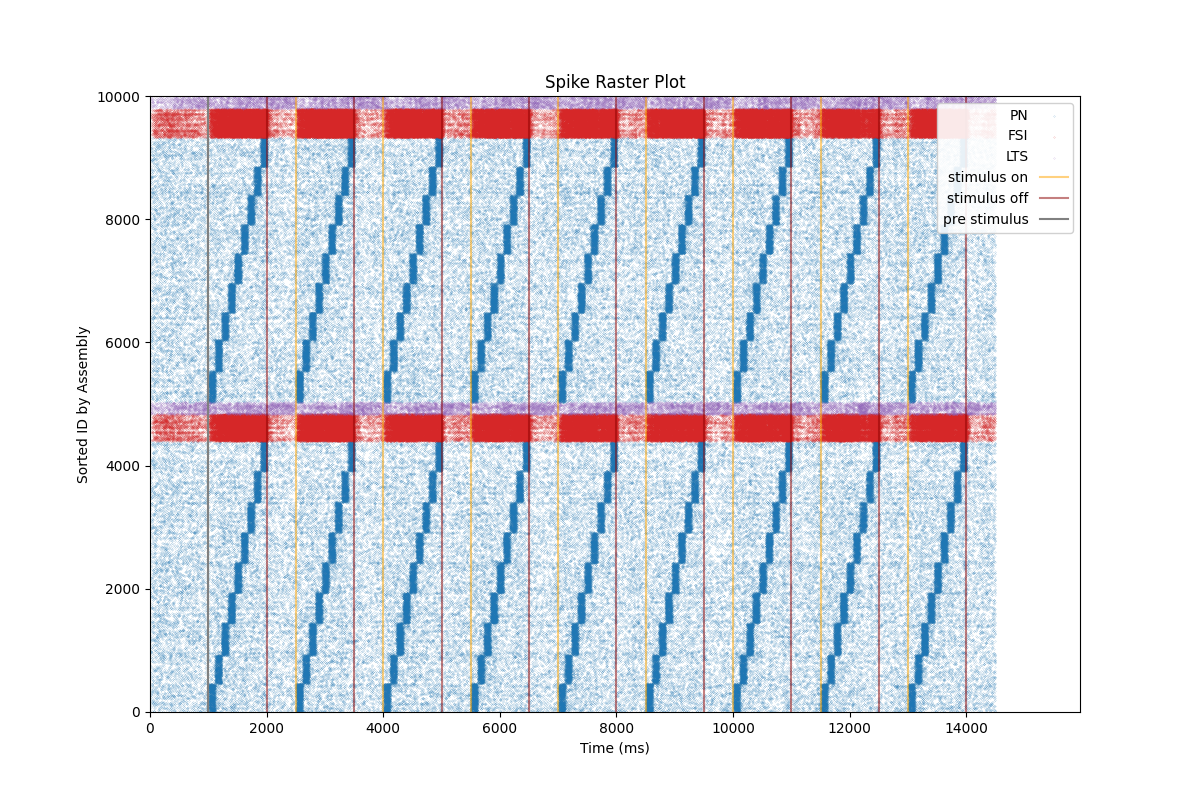
\includegraphics[width=\textwidth]{output/short-raster}
    \caption{Raster}
    \label{fig:short-raster}
  \end{subfigure}
  \caption{Firing Rate Analysis for Short Pulse}
\end{figure}

\begin{figure}[H]
    \centering
    \begin{subfigure}{.75\textwidth}
      \centering
      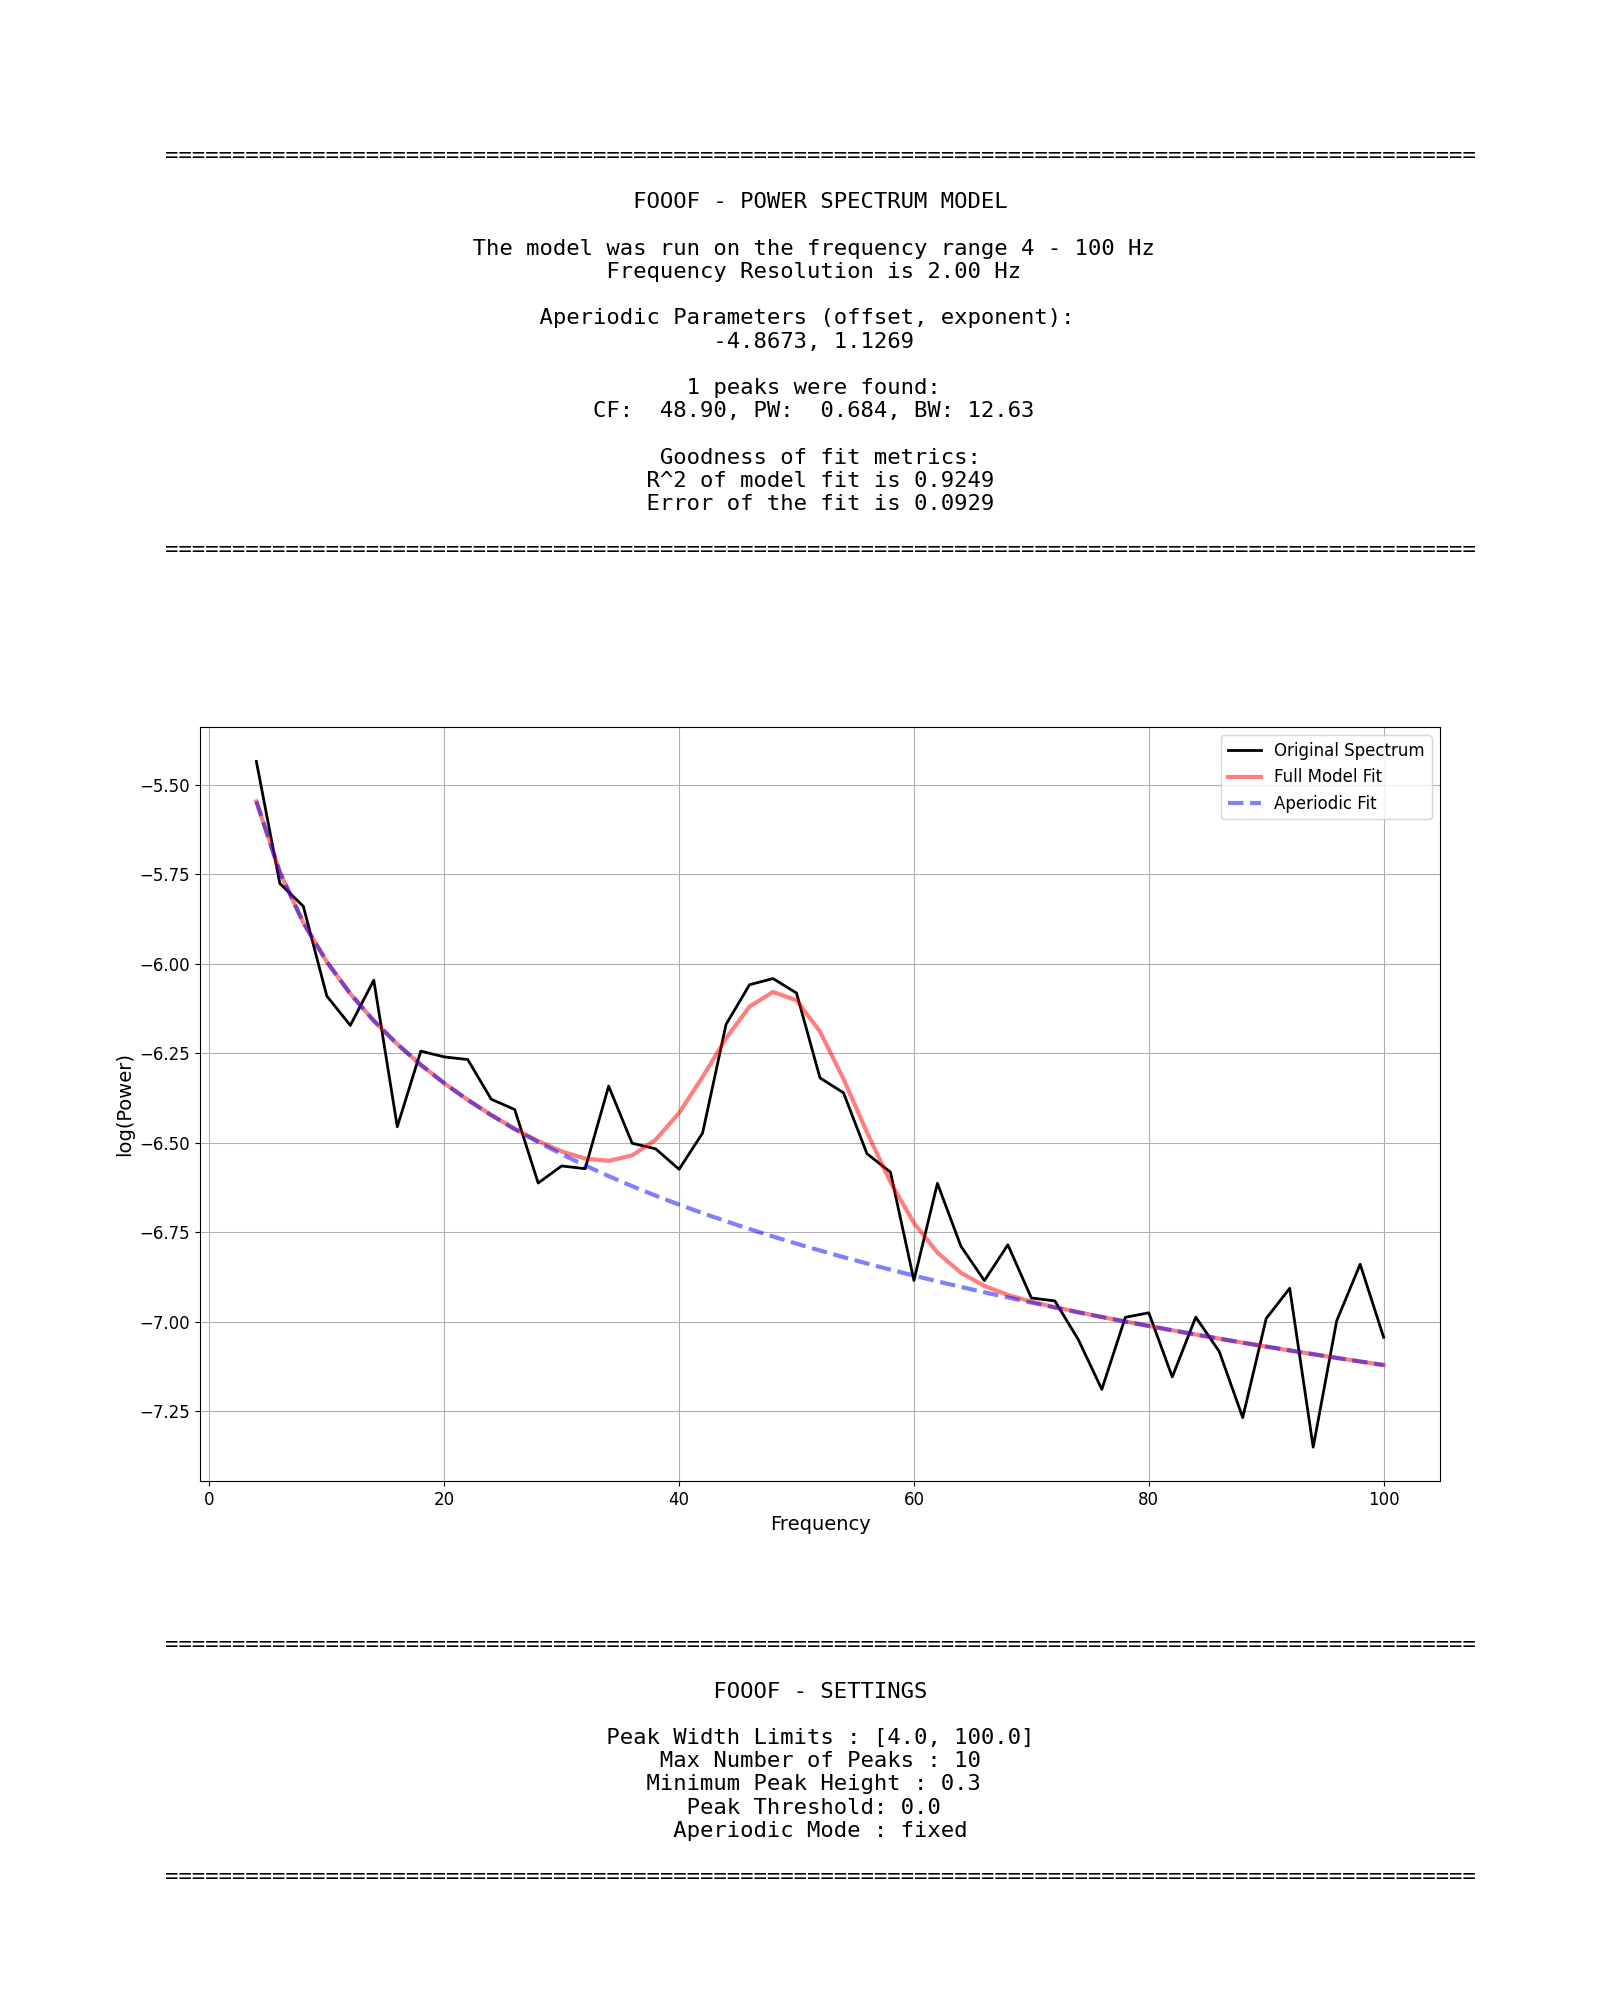
\includegraphics[width=\textwidth]{output/short-psd}
      \caption{Fooof Report}
      \label{fig:short-psd}
    \end{subfigure}
    \begin{subfigure}{.75\textwidth}
      \centering
      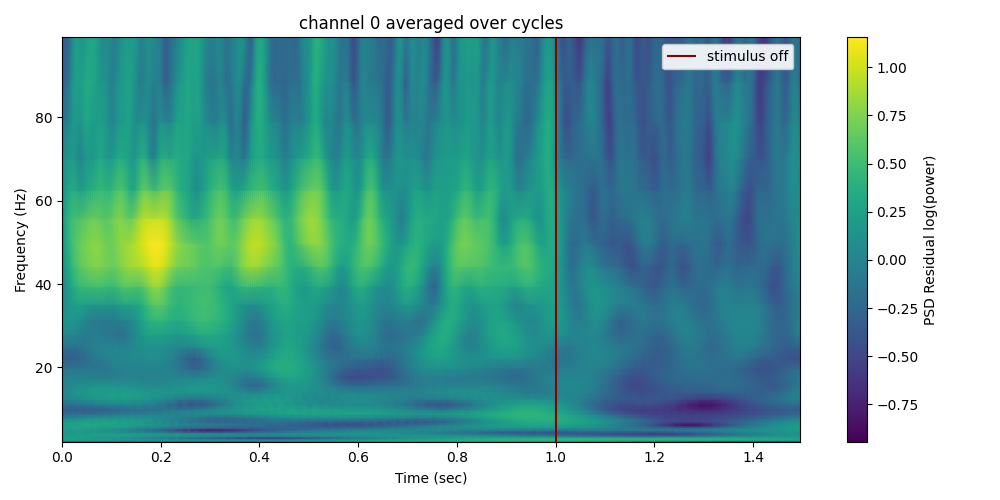
\includegraphics[width=\textwidth]{output/short-spectrogram}
      \caption{Spectrogram}
      \label{fig:short-spectrogram}
    \end{subfigure}
    \caption{Spectral Analysis for Short Pulse}
\end{figure}

\subsection*{Long Pulse}

\begin{figure}[H]
  \centering
  \begin{subfigure}{\textwidth}
    \centering
    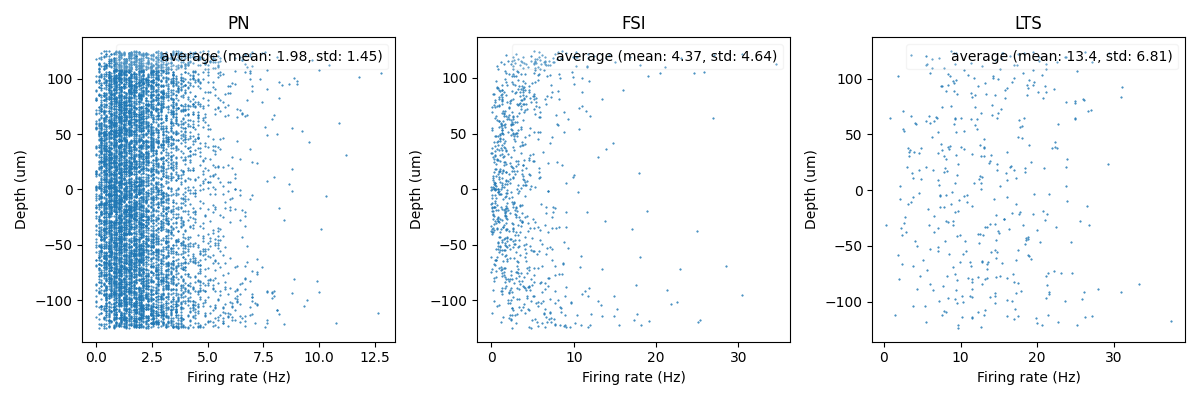
\includegraphics[width=\textwidth]{output/long-spikes}
    \caption{Firing Rate during Long Pulse}
    \label{fig:long-spikes}
  \end{subfigure}
  \begin{subfigure}{\textwidth}
    \centering
    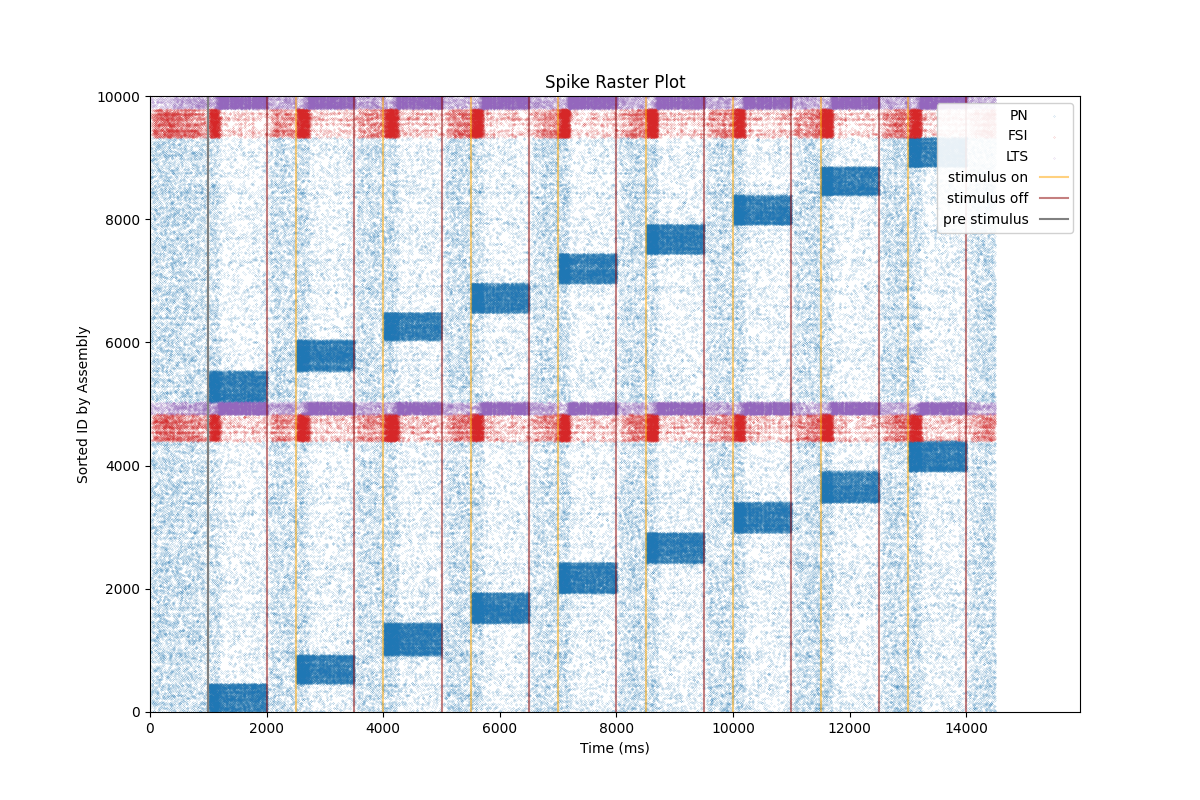
\includegraphics[width=\textwidth]{output/long-raster}
    \caption{Raster}
    \label{fig:long-raster}
  \end{subfigure}
  \caption{Firing Rate Analysis for Long Pulse}
\end{figure}

\begin{figure}[H]
    \centering
    \begin{subfigure}{.75\textwidth}
      \centering
      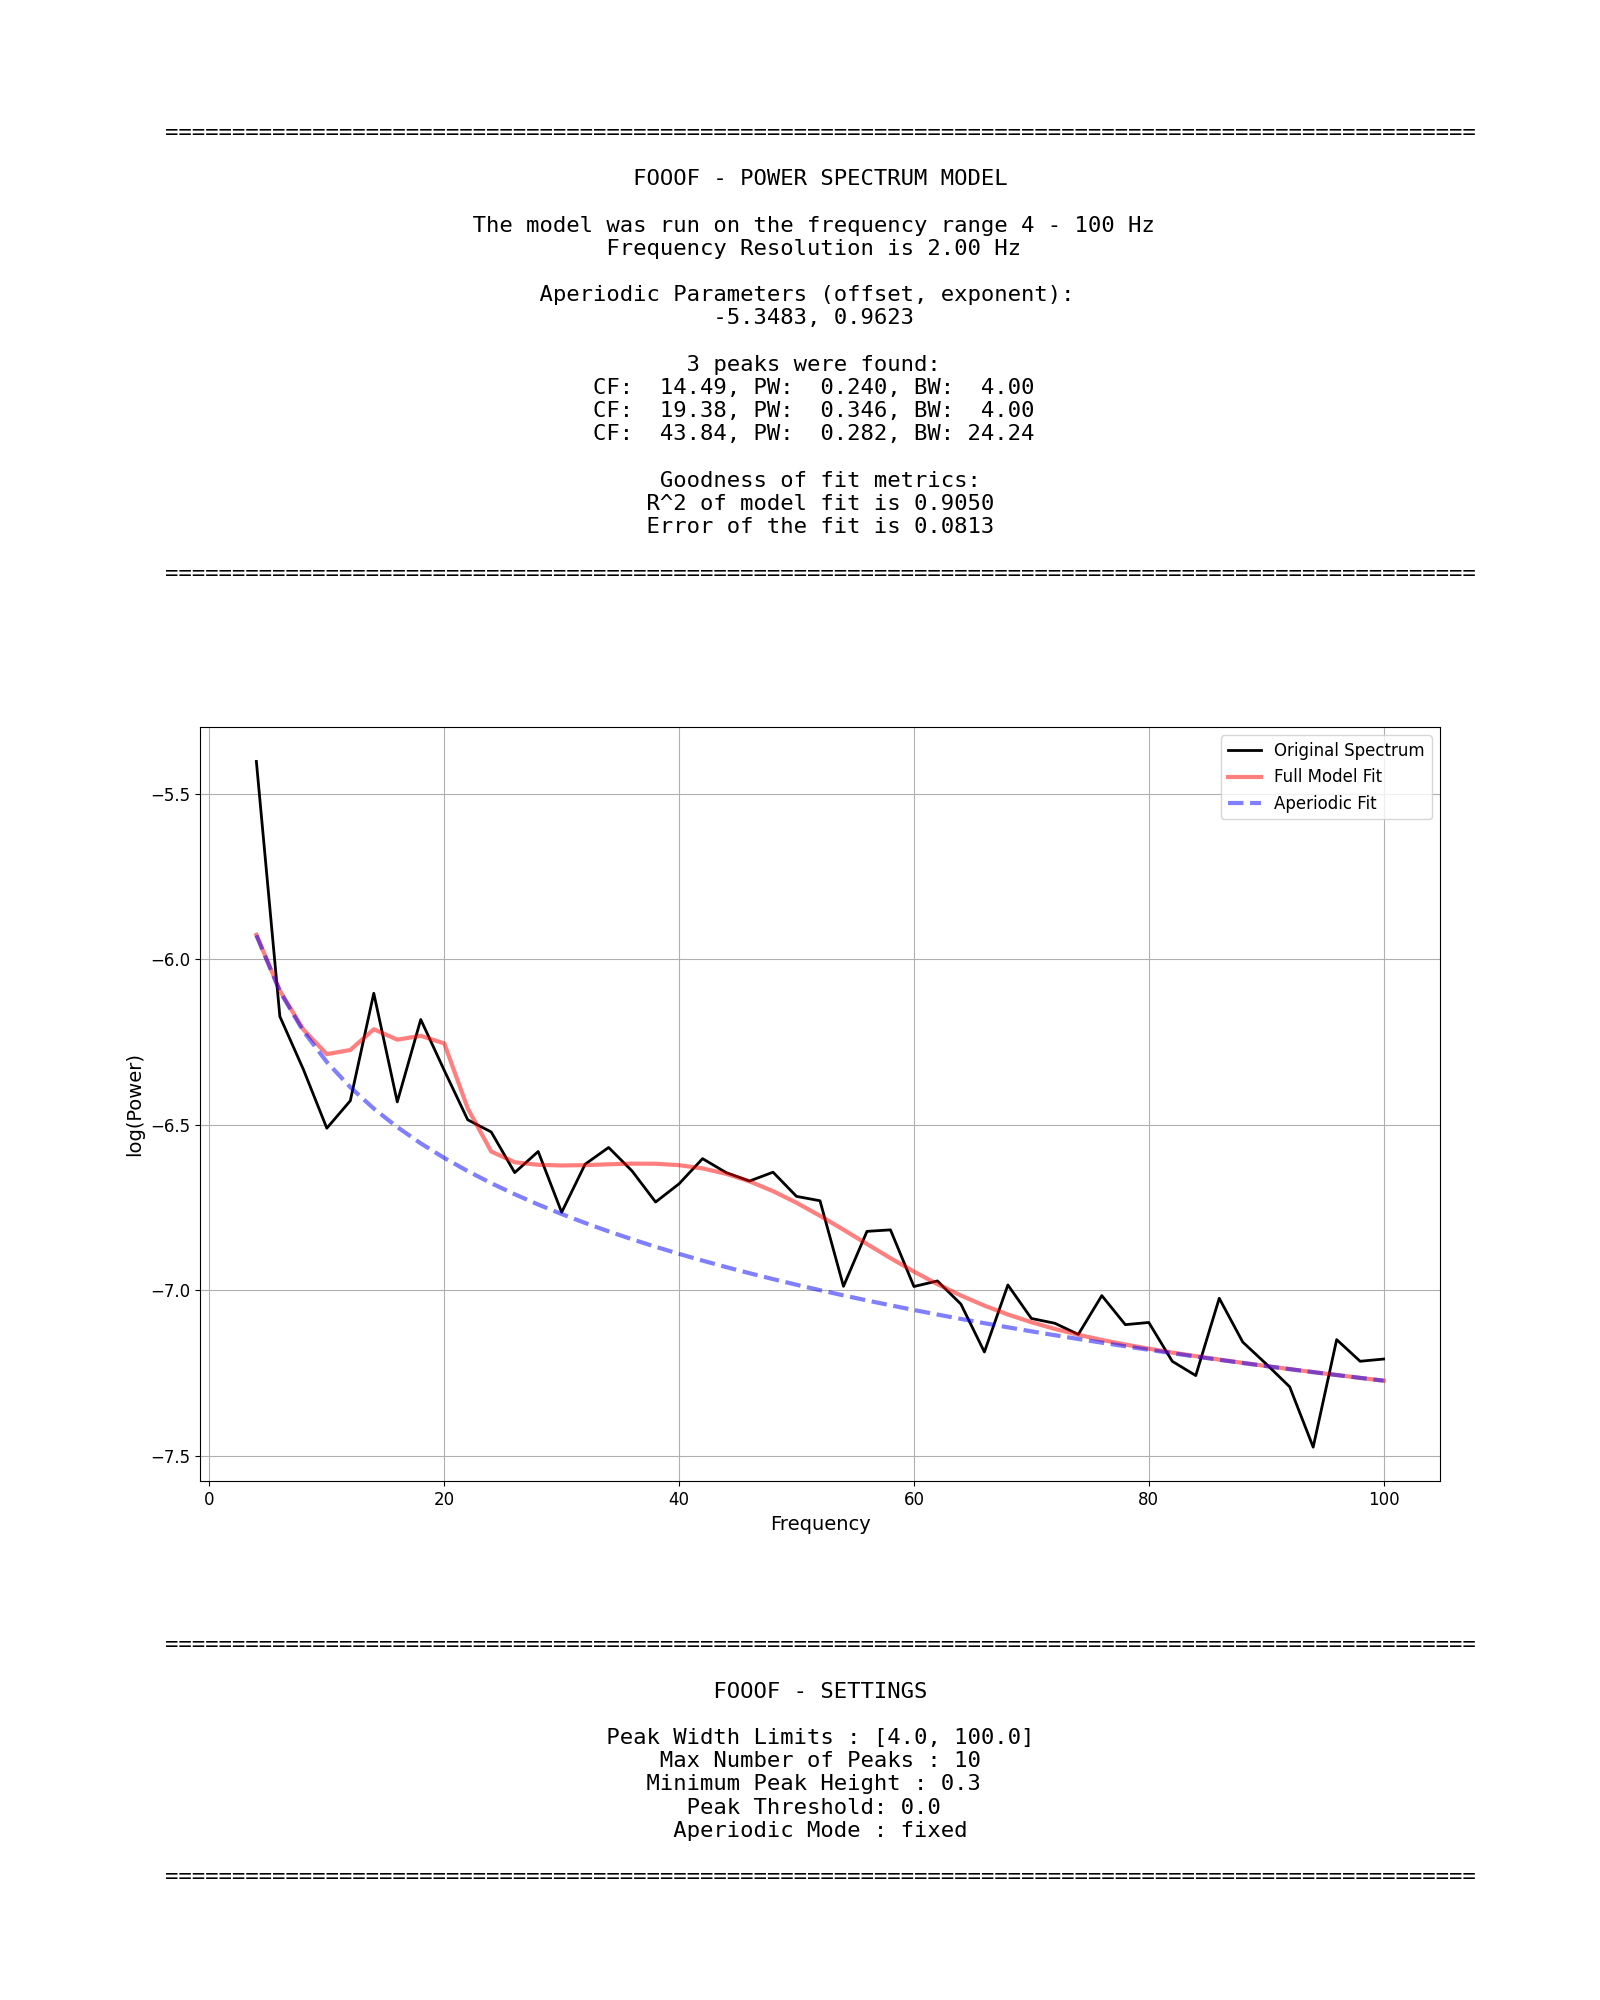
\includegraphics[width=\textwidth]{output/long-psd}
      \caption{Fooof Report}
      \label{fig:long-psd}
    \end{subfigure}
    \begin{subfigure}{.75\textwidth}
      \centering
      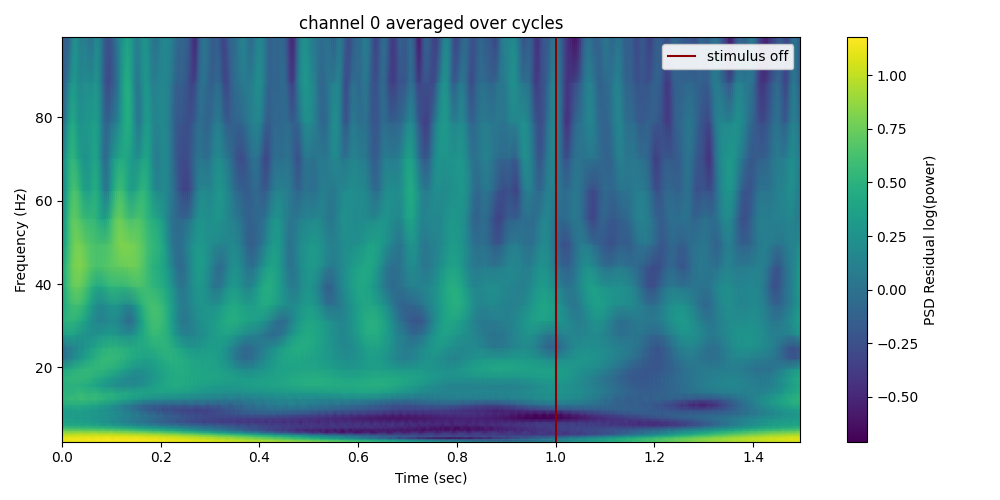
\includegraphics[width=\textwidth]{output/long-spectrogram}
      \caption{Spectrogram}
      \label{fig:long-spectrogram}
    \end{subfigure}
    \caption{Spectral Analysis for Long Pulse}
\end{figure}

\bibliographystyle{plain}
\bibliography{export} %bib is the file name for bib.bib it

\end{document}
